\documentclass{llncs}
\usepackage[utf8]{inputenc}
\usepackage{hyperref}
\usepackage[
 backend=biber,
 style=numeric,
 url=false,
 isbn=false,
 doi=false,
 bibencoding=utf8
	]{biblatex}

\usepackage[
  citations=true,
  hybrid=true
   ]{markdown}
\markdownSetup{
  renderers = {
    link = {\href{#2}{#1}}
  }
}

\addbibresource{main.bib}
\begin{document}
\title{VMEXT2: A Visual Wikidata aware content MathML Editor}

\author{
   Moritz Schubotz
}

\institute{
	\hspace{-0.15cm}
	Dept.~of Computer and Information Science,\\
	University of Konstanz, Box 76, 78464 Konstanz, Germany,\\
	\email{moritz.schubotz@uni-konstanz.de}
}

\maketitle

\begin{abstract}
VMEdit is a visual content MathML editor.
In the standard workflow parallel markup is generated from LaTeX input, which we visualize in expression tree form.
Then, the user alters the tree structure via drag and drop and links symbols to content dictionary entries.
In addition to the standard OpenMath content dictionaries, Wikidata items can be used as content symbols.
\end{abstract}

\keywords{MathML, VMEXT}
\begin{figure}[t]
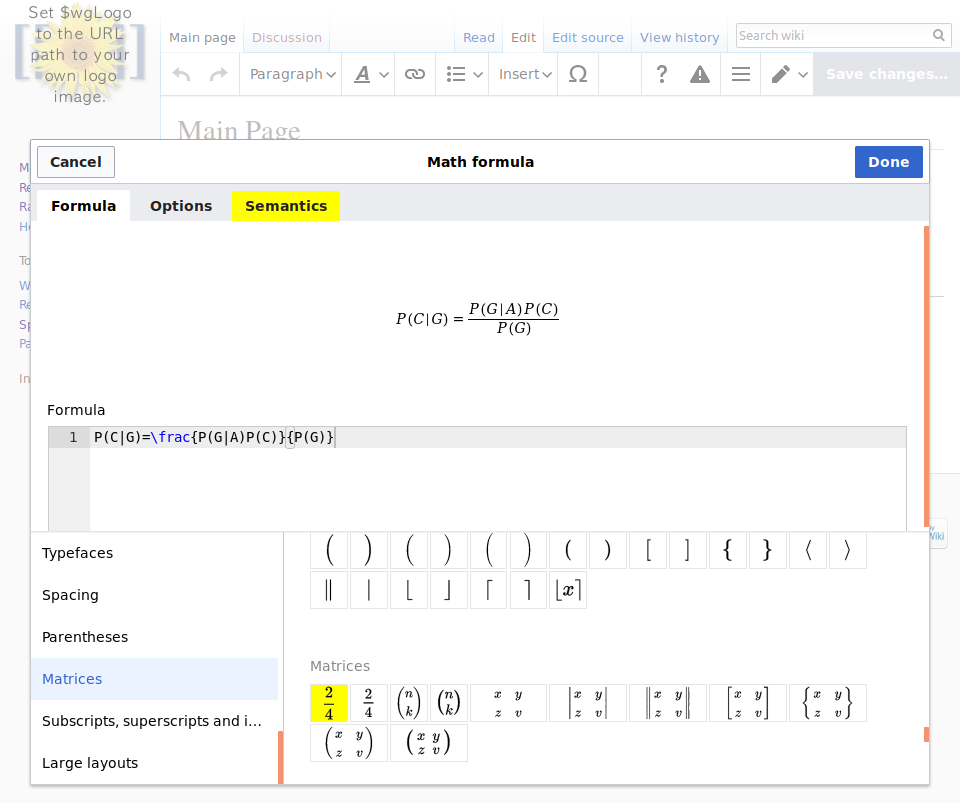
\includegraphics[width=\textwidth]{images/overview.png}
\caption{Math editing component of the Visual Editor.
 As of April 2018 users need either to know the {\LaTeX}-command for fraction or use the fraction tempate ($\frac{2}{4}$, hightlighted in yellow) and replace 2 by the nominator and 4 by the denominator of the formula.
 VMedit will improve this dialog by adding semantic intput as alternative in the top panel (Semantics, highlighted in yellow).}\label{fig.overview}
\end{figure}
\markdownInput{main.md}
\paragraph*{Acknowledgments} We thank the developers Ludwig Goohsen, Stefan Kaufhold, Jonas Kress, Vincent Stange and many others for their open source contributions.
 Furthermore, we thank the Wikimedia Foundation in particular Thalia Chan, Ed Sanders and James Forrester from the editing team for the development of the current VisualEditor for Math.
\printbibliography[keyword=primary]
\end{document}
